\begin{figure*}[htp]
    \centering
    \begin{subfigure}[b]{0.23\textwidth}
        \centering
        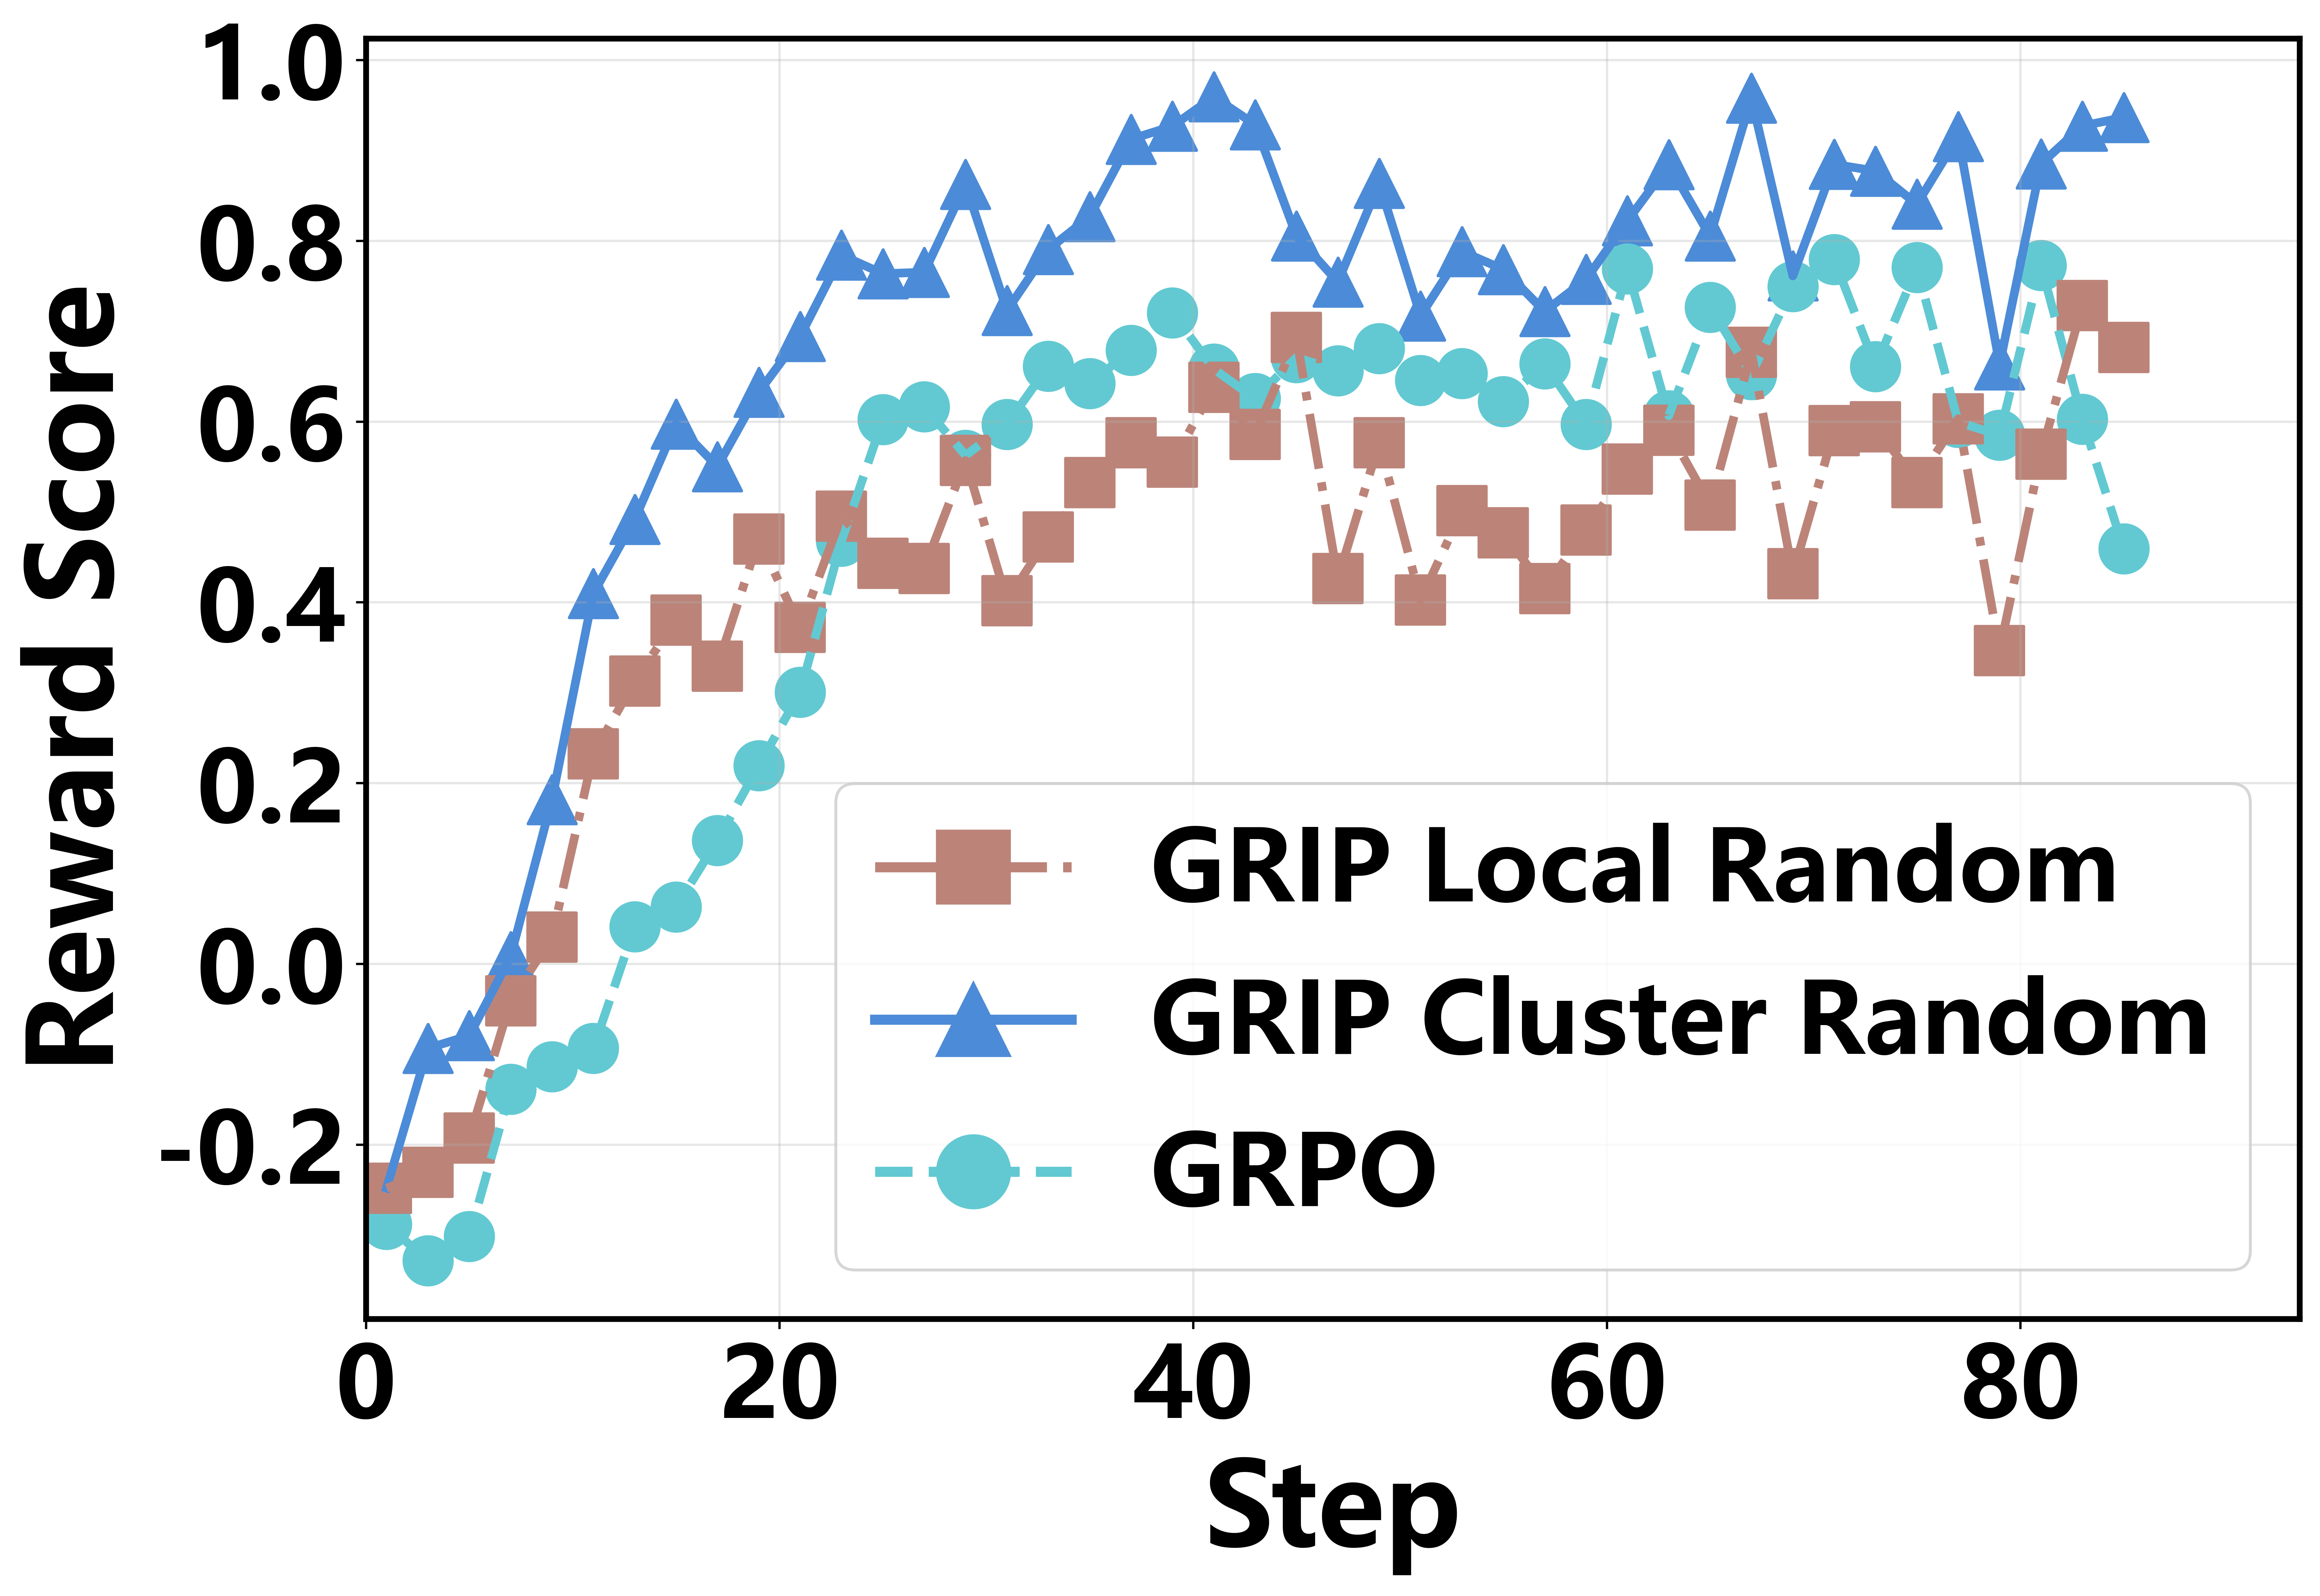
\includegraphics[width=\textwidth]{images/compare/GRIP_work.png}
        % \vspace{-0.1in}
        \caption{GRIP vs. GRPO}
        \label{fig:compare_a}
    \end{subfigure}
    \hfill
    \begin{subfigure}[b]{0.23\textwidth}
        \centering
        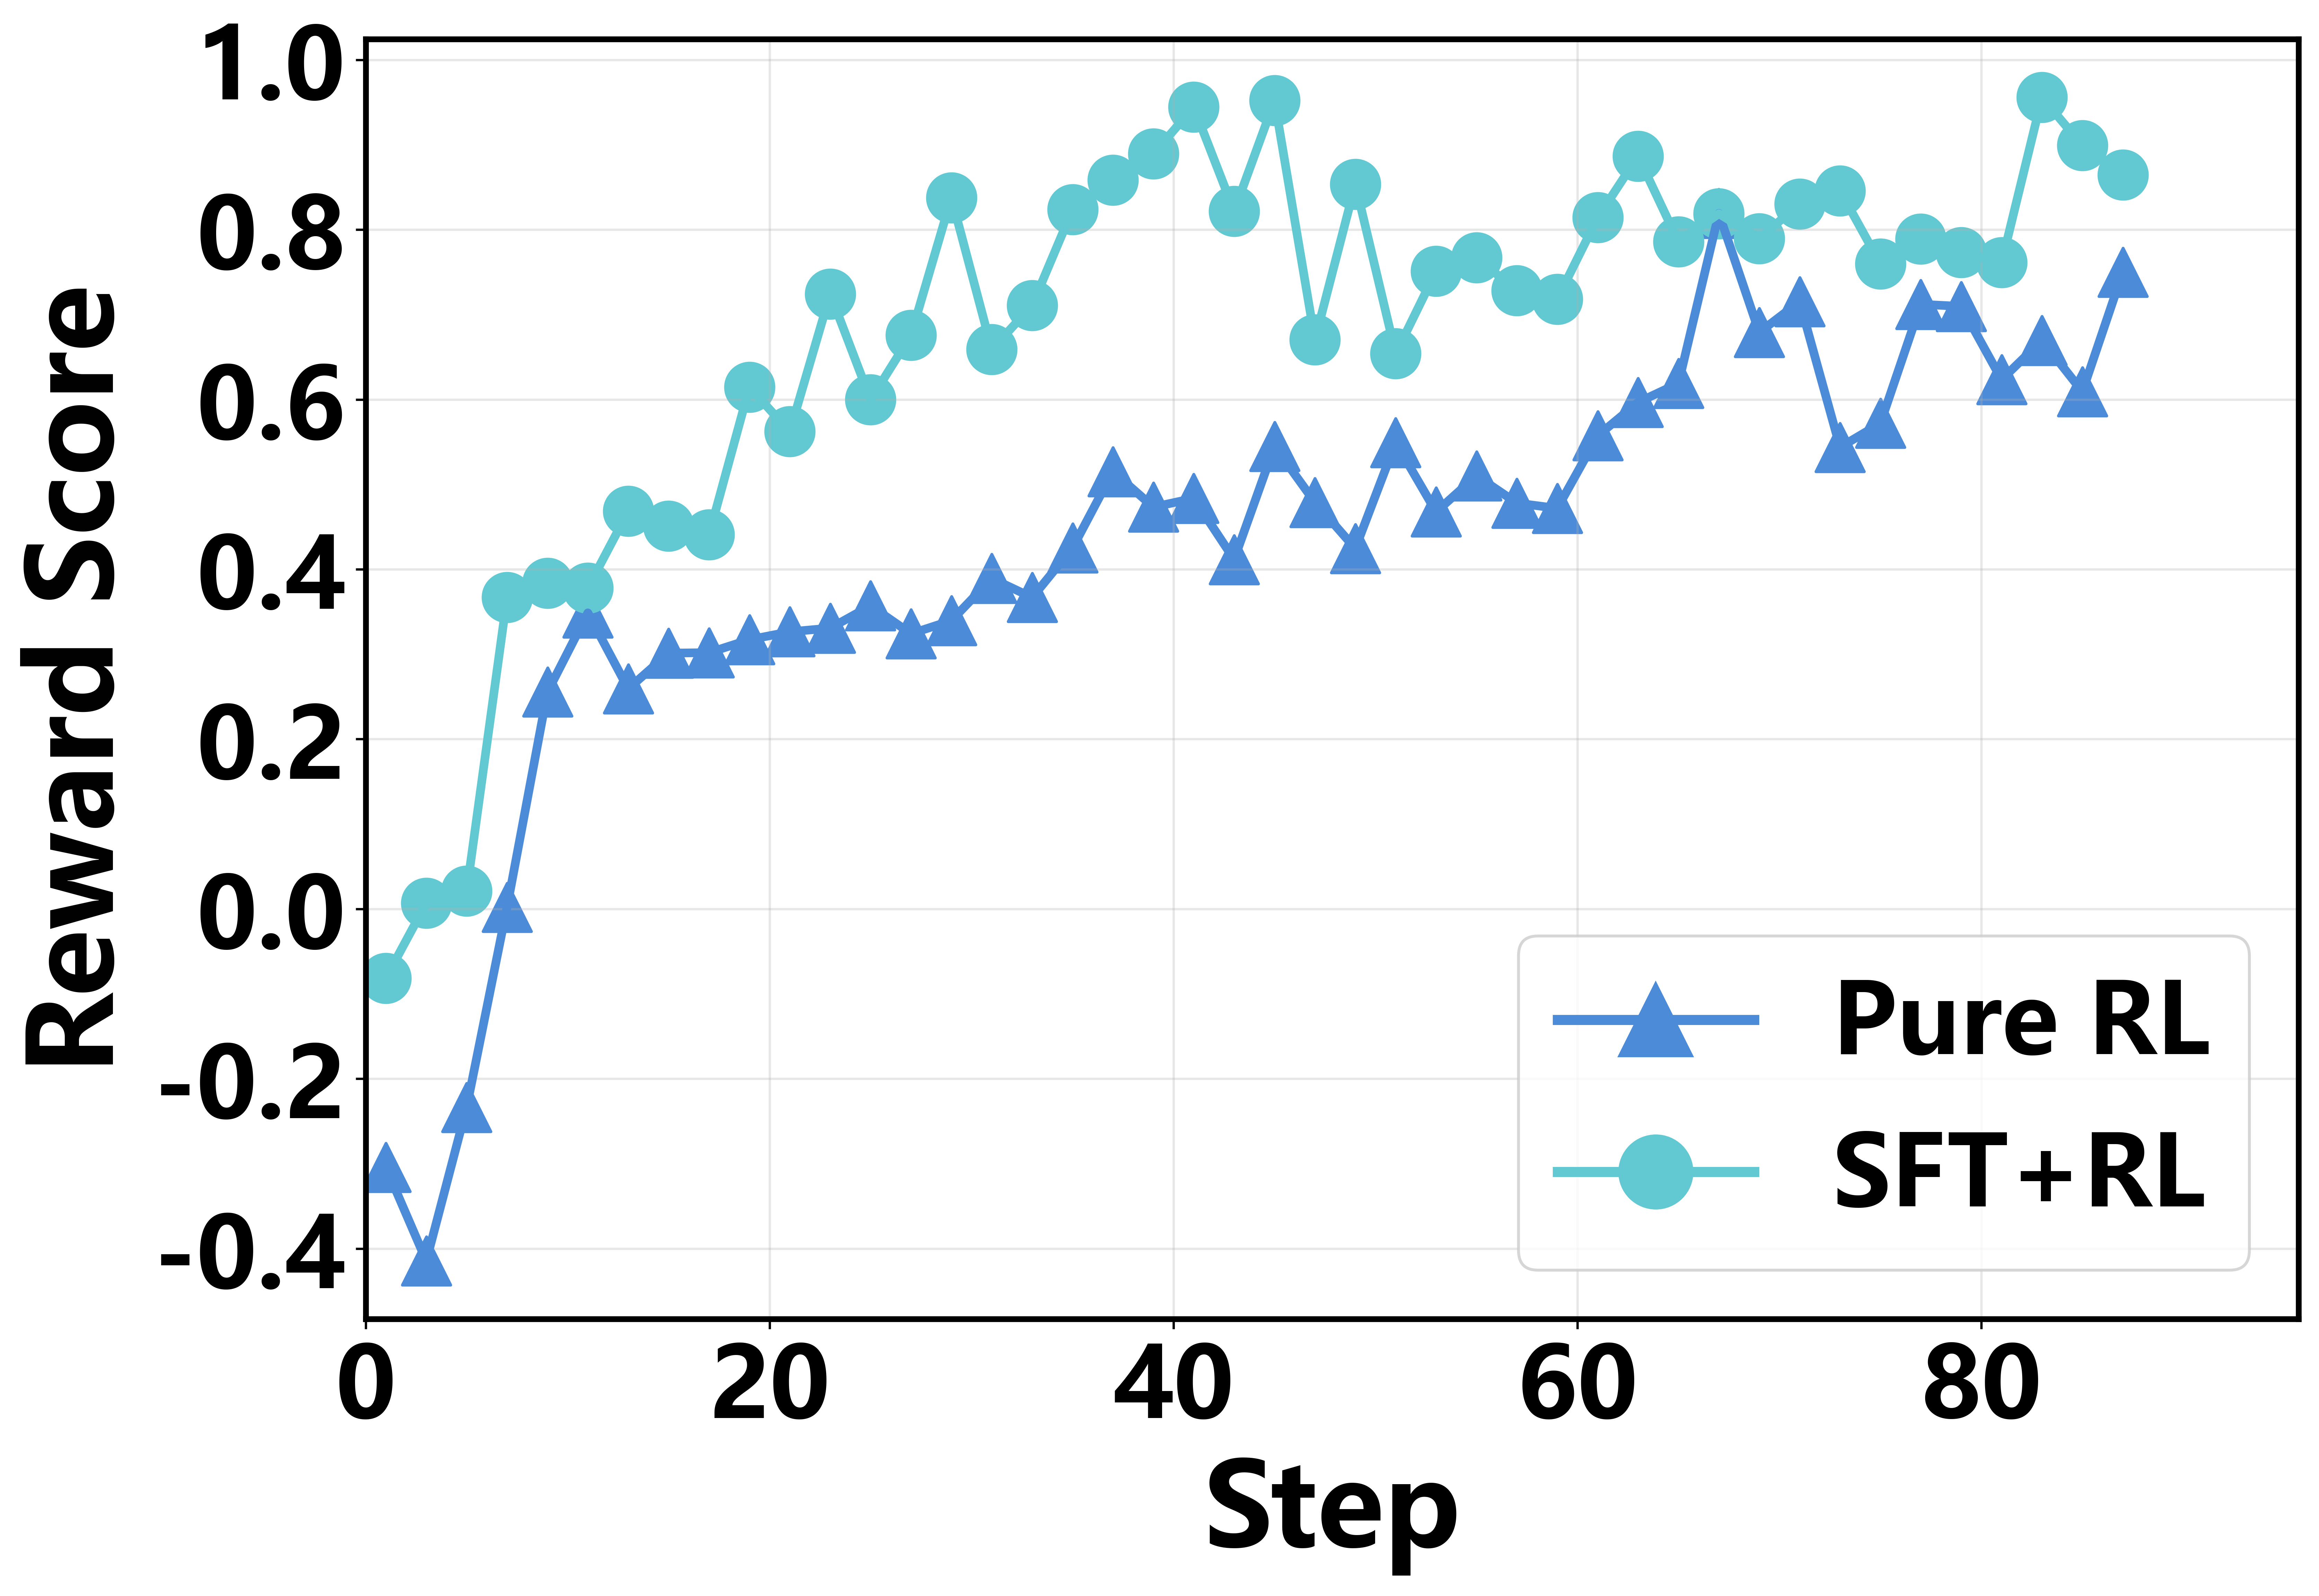
\includegraphics[width=\textwidth]{images/compare/SFT_RL.png}
        % \vspace{-0.1in}
        \caption{RL vs. SFT + RL}
        \label{fig:compare_b}
    \end{subfigure}
    \hfill
    \begin{subfigure}[b]{0.23\textwidth}
        \centering
        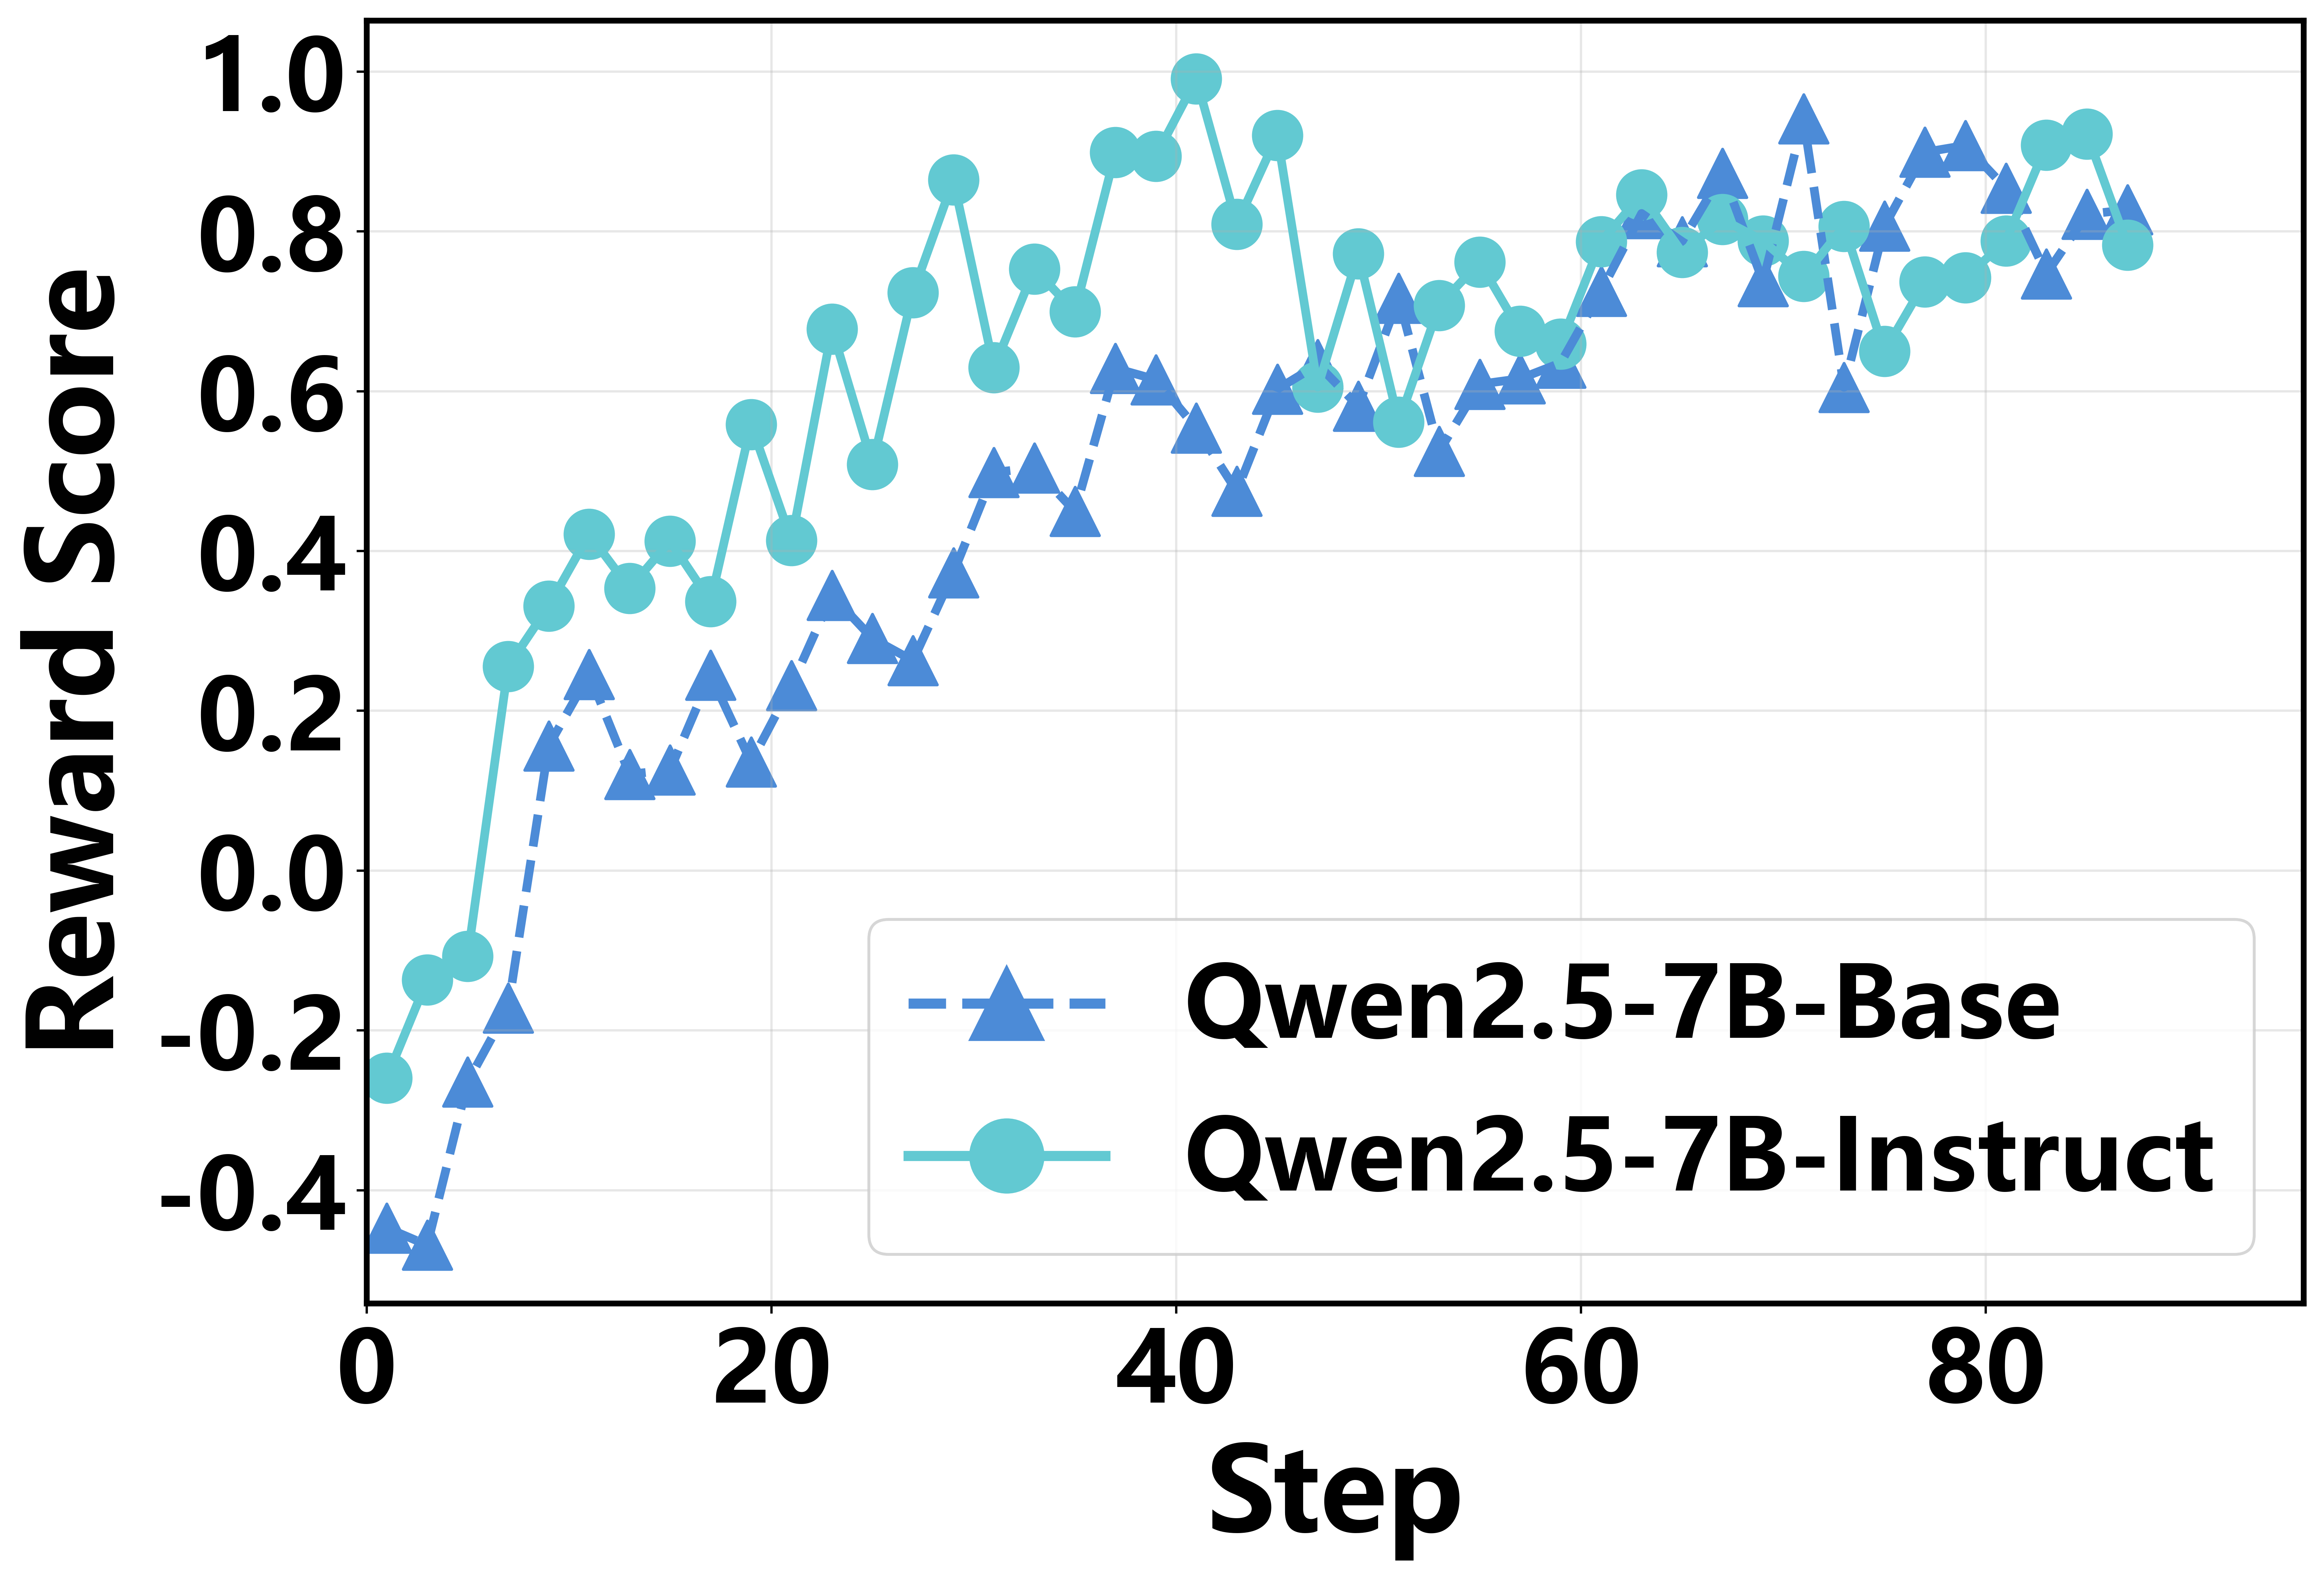
\includegraphics[width=\textwidth]{images/compare/Base_Instruct.png}
        % \vspace{-0.1in}
        \caption{Base vs. Instruct}
        \label{fig:compare_c}
    \end{subfigure}
    \hfill
    \begin{subfigure}[b]{0.23\textwidth}
        \centering
        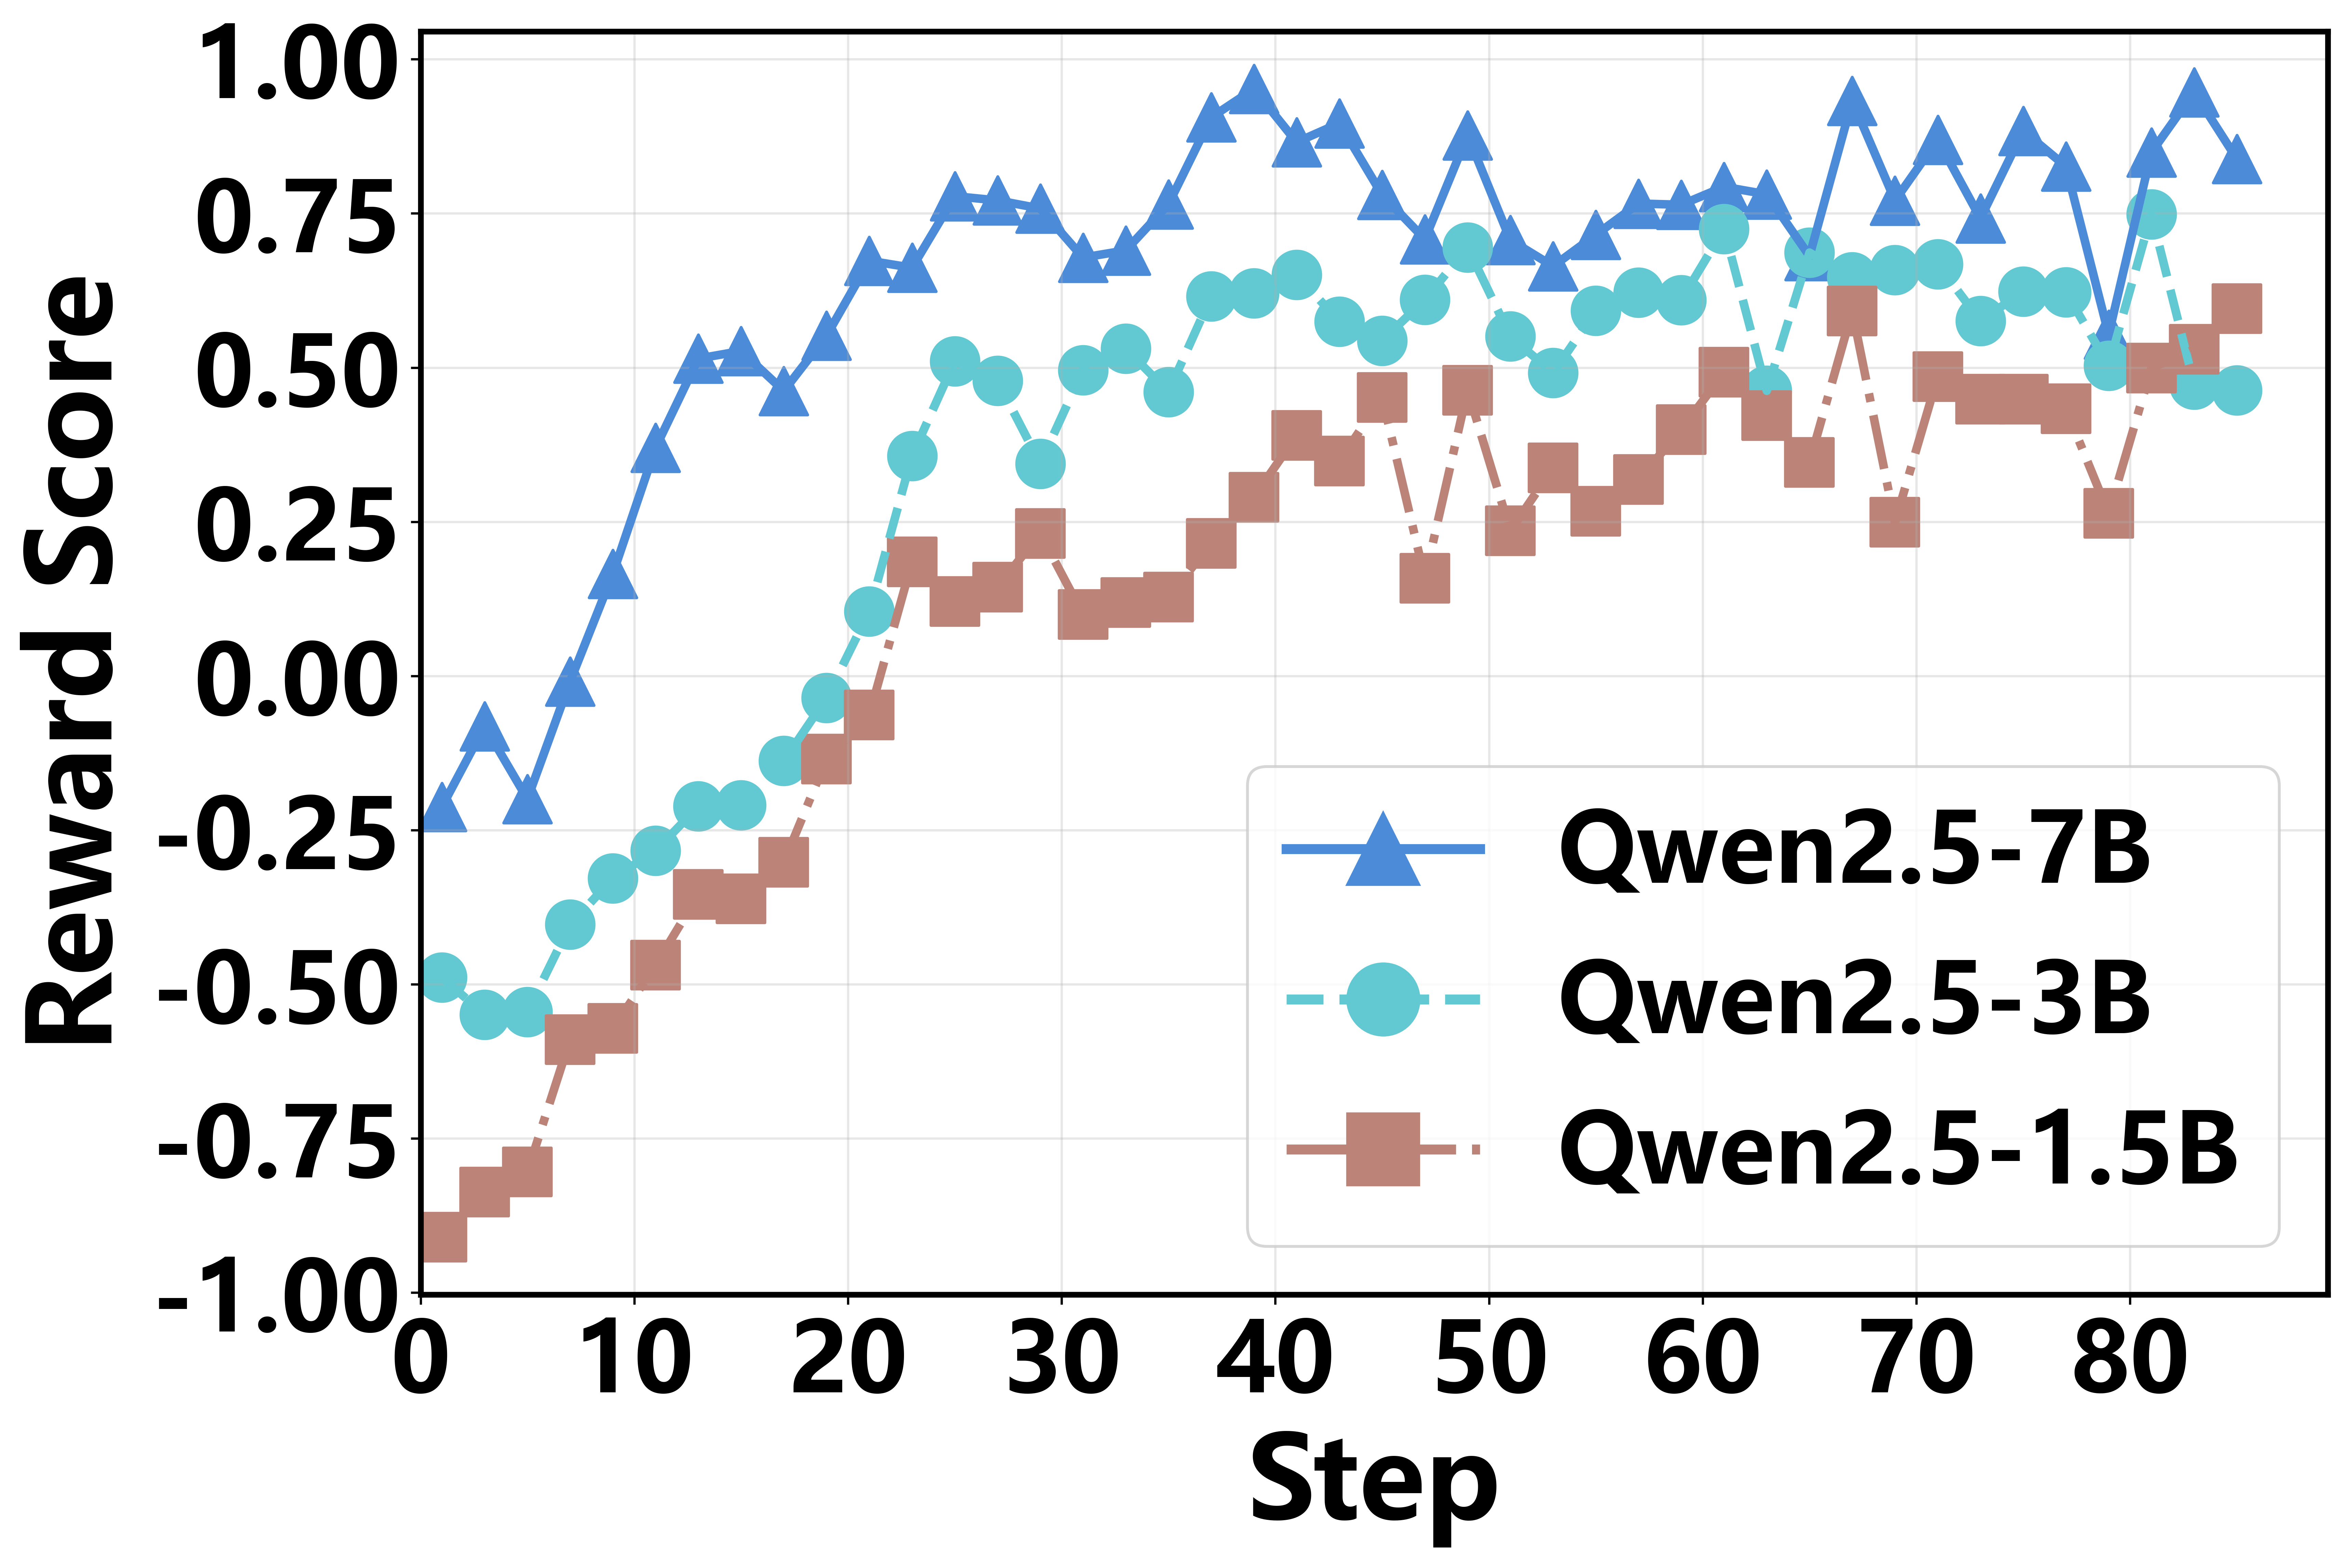
\includegraphics[width=\textwidth]{images/compare/model_scale.png}
        % \vspace{-0.1in}
        \caption{Model Scaling}
        \label{fig:compare_d}
    \end{subfigure}

    \caption{(a) GRIP vs. GRPO: GRIP converges faster with slightly higher final performance. (b) RL vs. SFT+RL: SFT+RL achieves faster initial convergence and superior final performance. (c) Base vs. Instruct: Instruct model enables faster early reward growth, though base model achieves higher final reward. (d) Model Scaling: Larger models achieve higher final rewards, indicating stronger time-series reasoning and forecasting capability.}
    \label{fig:compare}

\end{figure*}